% !TEX program = pdflatex
\RequirePackage[l2tabu, orthodox]{nag}
\documentclass{article}

% FONTS
\usepackage[T1]{fontenc}

% Replace default Latin Modern typewriter with its proportional counterpart
% http://www.tug.dk/FontCatalogue/lmoderntypewriterprop/
\renewcommand*\ttdefault{lmvtt}


%%% OPTION 1 - Fourier Math + New Century Schoolbook + ParaType Sans

% % Import Fourier Math (this imposes its own New Century Schoolbook type)
% % http://www.ctan.org/tex-archive/fonts/fouriernc/
% \usepackage{fouriernc}
% \usepackage{amsmath}
% % Replace with TeX Gyre Schola version of New Century Schoolbook (must scale!)
% % http://www.tug.dk/FontCatalogue/tgschola/
% \usepackage[scale=0.92]{tgschola}
% \usepackage[scaled=0.88]{PTSans}

%% OPTION 2 - MathDesign Math + Bitstream Charter + ParaType Sans

% Import MathDesign (this brings along Bitstream Charter)
% http://www.ctan.org/tex-archive/fonts/mathdesign/
\usepackage[bitstream-charter]{mathdesign}
\usepackage{amsmath}
\usepackage[scaled=0.92]{PTSans}


% %%% OPTION 3 - MTPRO 2 Math + Termes Times + ParaType Sans

% \usepackage{tgtermes}
% \usepackage{amsmath}
% \usepackage[subscriptcorrection,
%             amssymbols,
%             mtpbb,
%             mtpcal,
%             nofontinfo  % suppresses all warnings
%            ]{mtpro2}
% \usepackage{scalefnt,letltxmacro}
% \LetLtxMacro{\oldtextsc}{\textsc}
% \renewcommand{\textsc}[1]{\oldtextsc{\scalefont{1.10}#1}}
% \usepackage[scaled=0.92]{PTSans}

% GEOMETRY
\usepackage[
  paper  = letterpaper,
  left   = 1.65in,
  right  = 1.65in,
  top    = 1.0in,
  bottom = 1.0in,
  ]{geometry}

% COLOR
\usepackage[usenames,dvipsnames]{xcolor}
\definecolor{shadecolor}{gray}{0.9}

% SPACING and TEXT
\usepackage[final,expansion=alltext]{microtype}
\usepackage[english]{babel}
\usepackage[parfill]{parskip}
\usepackage{afterpage}
\usepackage{framed}

%redefine the leftbar environment to accept a width and coloring options
\renewenvironment{leftbar}[1][\hsize]
{%
  \def\FrameCommand
  {%
    {\color{Gray}\vrule width 3pt}%
    \hspace{10pt}%
    %\hspace{0pt}\fboxsep=\FrameSep\colorbox{black!10}%
  }%
  \MakeFramed{\hsize#1\advance\hsize-\width\FrameRestore}%
}%
{\endMakeFramed}

% define a paragraph header function
\DeclareRobustCommand{\parhead}[1]{\textbf{#1}~}

% EDITING
% line numbering in left margin
\usepackage{lineno}
\renewcommand\linenumberfont{\normalfont
                             \footnotesize
                             \sffamily
                             \color{SkyBlue}}
% ragged paragraphs in right margin
\usepackage{ragged2e}
\DeclareRobustCommand{\sidenote}[1]{\marginpar{
                                    \RaggedRight
                                    \textcolor{Plum}{\textsf{#1}}}}
% paragraph counter in right margin
\newcommand{\parnum}{\bfseries\P\arabic{parcount}}
\newcounter{parcount}
\newcommand\p{%
    \stepcounter{parcount}%
    \leavevmode\marginpar[\hfill\parnum]{\parnum}%
}
% paragraph helper
\DeclareRobustCommand{\PP}{\textcolor{Plum}{\P} }

% COUNTERS
\renewcommand{\labelenumi}{\color{black!67}{\arabic{enumi}.}}
\renewcommand{\labelenumii}{{\color{black!67}(\alph{enumii})}}
\renewcommand{\labelitemi}{{\color{black!67}\textbullet}}

% FIGURES
\usepackage{graphicx}
\usepackage[labelfont=bf]{caption}
\usepackage[format=hang]{subcaption}

% TABLES
\usepackage{booktabs}

% ALGORITHMS
\usepackage[algoruled]{algorithm2e}
\usepackage{listings}
\usepackage{fancyvrb}
\fvset{fontsize=\normalsize}

% BIBLIOGRAPHY
\usepackage{natbib}

% HYPERREF
\usepackage[colorlinks,linktoc=all]{hyperref}
\usepackage[all]{hypcap}
\hypersetup{citecolor=BurntOrange}
\hypersetup{linkcolor=MidnightBlue}
\hypersetup{urlcolor=MidnightBlue}

% CLEVEREF must come after HYPERREF
\usepackage[nameinlink]{cleveref}

% ACRONYMS
\usepackage[acronym,smallcaps,nowarn]{glossaries}
% \makeglossaries

% COLOR DEFINITIONS
\newcommand{\red}[1]{\textcolor{BrickRed}{#1}}
\newcommand{\orange}[1]{\textcolor{BurntOrange}{#1}}
\newcommand{\green}[1]{\textcolor{OliveGreen}{#1}}
\newcommand{\blue}[1]{\textcolor{MidnightBlue}{#1}}
\newcommand{\gray}[1]{\textcolor{black!60}{#1}}

% LISTINGS DEFINTIONS
\lstdefinestyle{mystyle}{
    commentstyle=\color{OliveGreen},
    keywordstyle=\color{BurntOrange},
    numberstyle=\tiny\color{black!60},
    stringstyle=\color{MidnightBlue},
    basicstyle=\ttfamily,
    breakatwhitespace=false,
    breaklines=true,
    captionpos=b,
    keepspaces=true,
    numbers=left,
    numbersep=5pt,
    showspaces=false,
    showstringspaces=false,
    showtabs=false,
    tabsize=2
}
\lstset{style=mystyle}


\DeclareRobustCommand{\mb}[1]{\ensuremath{\boldsymbol{\mathbf{#1}}}}

\DeclareMathOperator*{\argmax}{arg\,max}
\DeclareMathOperator*{\argmin}{arg\,min}

\DeclareRobustCommand{\KL}[2]{\ensuremath{\textrm{KL}\left(#1\;\|\;#2\right)}}

\newcommand{\mbx}{\mathbold{x}}
\newcommand{\mbX}{\mbf{X}}

\newcommand{\mbz}{\mathbold{z}}

\newcommand{\mbI}{\mbf{I}}

\newcommand{\mbZ}{\mbf{Z}}
\newcommand{\mbL}{\mbf{L}}

\newcommand{\mbtheta}{\mathbold{\theta}}
\newcommand{\mbTheta}{\mathbold{\Theta}}
\newcommand{\mbomega}{\mathbold{\omega}}
\newcommand{\mbOmega}{\mathbold{\Omega}}
\newcommand{\mbsigma}{\mathbold{\sigma}}
\newcommand{\mbSigma}{\mathbold{\Sigma}}

\newcommand{\mblambda}{\mathbold{\lambda}}
\newcommand{\mbgamma}{\mathbold{\gamma}}
\newcommand{\mbzeta}{\mathbold{\zeta}}
\newcommand{\mbeta}{\mathbold{\eta}}
\newcommand{\mbbeta}{\mathbold{\beta}}
\newcommand{\mbphi}{\mathbold{\phi}}
\newcommand{\mbmu}{\mathbold{\mu}}
\newcommand{\mbrho}{\mathbold{\rho}}

\newcommand\dif{\mathop{}\!\mathrm{d}}
\newcommand{\diag}{\textrm{diag}}
\newcommand{\supp}{\textrm{supp}}

\newcommand{\E}{\mathbb{E}}
\newcommand{\Var}{\mathbb{V}\textrm{ar}}

\newcommand{\bbN}{\mathbb{N}}
\newcommand{\bbZ}{\mathbb{Z}}
\newcommand{\bbR}{\mathbb{R}}
\newcommand{\bbS}{\mathbb{S}}

\newcommand{\cL}{\mathcal{L}}

\newcommand{\cN}{\mathcal{N}}
\newcommand{\Gam}{\textrm{Gam}}
\newcommand{\InvGam}{\textrm{InvGam}}

\newacronym{KL}{kl}{Kullback-Leibler}
\newacronym{ELBO}{elbo}{\emph{evidence lower bound}}
\newacronym{POPELBO}{pop-elbo}{\emph{population evidence lower bound}}

\newacronym{SVI}{svi}{stochastic variational inference}
\newacronym{BUMPVI}{bump-vi}{bumping variational inference}

\newacronym{GMM}{gmm}{Gaussian mixture model}
\newacronym{LDA}{lda}{latent Dirichlet allocation}

\newacronym{SUTVA}{sutva}{stable unit treatment value assumption}


% \linenumbers

\title{Trygve's Problem}
\author{Jackson Loper}

\usepackage{amsthm}
\newtheorem{thm}{Theorem}
\newtheorem{conj}{Conjecture}

\begin{document}
\maketitle

\begin{description}
  \item[Status] Designed estimator, showed result to Allen people, they seem happy
  \item[Todo] Prove consistency, try on other Allen datasets, sample uniformly from possible set
\end{description}


\section{Overview}

When many different measurement tools are applied, how can we best combine information from the different different tools?  If we can apply various measurement tools to the same specimens, we can at least begin to understand how the tools they are related.  We call this ``joint measurement.''  However, the challenge is compounded when joint measurement is unavailable.  For example, consider the case that the measurement tools are destructive.  After processing a neuron with a given single-cell rna sequencing technique, we cannot generally go back and process that same neuron with a different technique.  This is because the measurement technique destroys the original neuron.  This means we can never see \emph{both measurements} for the same cell, side by side.  How, then, can we ever hope to understand how the different measurements relate to each other?

In this paper, we hope to shed some light on this this basic mathematical question.  It has many applications in the sciences.  For example:

\begin{itemize}

\item Different tools may teach us different things, and we need to combine tools
to learn everything we can.  Let $A,B$ denote two different quantities of interest about cells (e.g. morphology and gene expression).   Let us say one tool enables us to measure $A$ and another tool to measure $B$.  We would like
to be able to say something about what morphologies are associated with what gene expressions.  

\item Two labs may used different methods, but may wish to pool results.  Each lab looks at the other
lab's data and asks themselves "what would their data have looked like if they had used our method?"  When
they find they don't know the answer, it greatly complicates collaboration.

\item One may attempt to cluster the data.  It is simple to cluster the data from one technique, and cluster the data
from another technique -- but how can we know how those clusters correspond to one another?  

\end{itemize}

In this work we show that it is indeed sometimes possible to get useful and statistically rigorous bounds for these kinds of questions, even when joint measurements are unavailable.   

In particular, we consider the case that we can obtain samples from a variety of subpopulations.  If we can assume that the \emph{relationship} between the measurements is the same in each subpopulation, we can use these samples to learn something about that relationship -- even though we never see both measurements for any single member of the population.  

We apply our method to single cell RNA data.  We show how different clusterings from different single cell RNA modalities can be connected.  Our method yields results which are generally consistent with the scientist's understanding of the data and clusters, but also reveal potential gaps which could be important for further study.

\section{Mathematical formulation}

Mathematically, we formulate our model as follows:

\begin{itemize}
\item Let us say we have $n+m$ individual members of a population.  These could be cells, humans, or whatever the smallest sample unit may be for a given problem.
\item For each individual member, we have some readily observable features by which we can group the members, such as the size of a cell, where an individual lives, or some other basic information.  We designate these features as $\ell_i$ for the $i$th individual.
\item For the first $n$ members, we have made an observation using the first technique.  This gives us the values $X_1 \cdots X_n$.
\item The last $m$ members were observed using the second technique.  This gives us the values $Y_{n+1} \cdots Y_{n+m}$.
\end{itemize}

For simplicity, we here assume that $\ell_i,X_i,Y_i$ take values in finite sets, $\Omega_\ell,\Omega_X,\Omega_Y$.  Extensions to more general cases should be straightforward, but we must leave them to future work.  

We further posit a set of \emph{counterfactual} variables -- variables which could not ever be obtained in practice, but which help us organize our thinking.  These are sometimes referred to as "potential outcomes"  (cf. \cite{rubin2005causal}).

\begin{itemize}
\item Let $Y_1 \cdots Y_n$ denote the observations we \emph{would have gotten} if we had applied the second technique to the first $n$ members.
\item Let $X_{n+1} \cdots X_n$ denote the observations we would have gotten if we had applied the first technique to the last $m$ members. 
\end{itemize}

Our main assumption is that 

\begin{equation}
\mathbb{P}(X_i=x,Y_i=y|L_i=\ell)=p^*(x_i|\ell_i)q^*(y_i|x_i)
\end{equation}

for some distributions $p^*,q^*$.  Moreover, we assume that the vectors $\{(p^*(x_1|\ell)\cdots p^*(x_n|\ell))\}_\ell$ are linearly independent.  If this seems unlikely, it may make sense to collapse similar values of $\ell$ together.

The validity of these assumptions for a given situation should be closely contemplated.  There are several key questions to answer when deciding whether this assumption is applicable.  Does the process by which samples are gathered gathered depend only upon $\ell$?  In particular, is it not at all statistically related to which measurement technique was  applied, except through $\ell$?  Are the particular measurement biases of both techniques the same for every value of $\ell$?  Is the statistical relationship between the quantities being measured by the two techniques the same for every value of $\ell$?\footnote{Note that this is automatically true if both techniques are measuring the same thing.  More generally, if two techniques have something that they both measure, we can restrict attention to that one common phenomenon.}  If the answer to all of these questions is yes, the assumption that $(X_i,Y_i)$ is drawn from $p(x_i|\ell_i)p(y_i|x_i)$ may apply.

We can now articulate our goal.  Informally, our goal is to see what we can understand about the relationship between the observations $X_i$ from one measurement modality and the other measurement modality $Y_i$.  Ideally, we would like to learn the distribution $p^*(y_i|x_i)$.  Unfortunately, given the limitations of the data, this may not be possible.  Instead, we articulate a slightly less amibtious goal: to put \emph{bounds} on $q(y_i|x_i)$.  Specifically, we will seek to produce $\hat u_1(y|x),\hat u_2(y|x)$ such that

\begin{equation}\label{eq:ubound}
\hat u_1(y|x) \leq q^*(y|x) \leq \hat u_2(y|x)
\end{equation}

with high probability.  In particular, we define

\begin{align*}
\Theta^* &\triangleq\left\{q:\ \sum_x p^*(x|\ell) q^*(y|x) =\sum_x p^*(x|\ell)q^*(y|x), \forall \ell,y\right\}\\ 
u_1^*(y|x) &= \inf_{q\in\Theta^*} \{q(y|x)\} \\
u_2^*(y|x) &= \sup_{q\in\Theta^*} \{q(y|x)\}
\end{align*}

Then obviously $u_1^*(y|x) \leq q^*(y|x)\leq u_2^*(y|x)$ is a valid bound.  Moreover, given the data and assumptions we have, it is as tight a bound as is possible to make (indeed, we could not hope to distinguish between any two $q_1,q_2 \in \Theta^*$, since they yield the same distributions on what we can observe).

Thus, our mathematical task to to attempt to find estimators for $u_1^*,u_2^*$, which will allow us to bound the values of $q^*(y|x)$, and thus understand something about the relationship between the two measurements, $X$ and $Y$.

\section{Mathematical solution}

To produce useful bounds on $q^*(y|x)$, we first estimate

\begin{itemize}
\item $p^*$ using the empirical distribtion of the observations $\{X_i\}$, $\hat p(x|\ell)$
\item $h^*(y|\ell)\triangleq \sum_x p^*(x|\ell)q^*(y|\ell)$ using the empirical distribtion of $\{Y_i\}$, $\hat h(y|\ell)$
\end{itemize}

These empirical distributions may not be quite consistent with the original assumption that the distribution of $X,Y|\ell$ may be written as $p^*(x|\ell)q^*(y|x)$.  In particular, it may be that there is \emph{no} value of $q$ such that $\sum_x \hat p(x|\ell) q(y|x) = \hat h(y|\ell)$.  There may also be many such values.  We satisfy ourselves with finding a somewhat good fit for $q$.  Let $N_{X,\ell}=\#\{i\leq n:\ \ell_i=\ell\},N_{Y,\ell}=\#\{i> n:\ \ell_i=\ell\}$.  We take

\begin{equation}
\hat q = \argmax_q \sum_\ell N_{Y,\ell}\sum_{y}\hat h(y|\ell)\log\left(\sum_{x}\hat p(x|\ell)q(y|x)\right) + \kappa \sum_{xy} \log q(y|x)
\end{equation}

Note in the second term we apply an entropic penalty to $q$.  This is both necessary to ensure that $\hat q$ is uniquely defined in terms of $\hat q,\hat h$, as well as a useful regularization. This regularization pushes us slightly towards uniform distributions, which makes sense if we believe that $q(y|x)>0$  for each $x,y$.  Other regularizations could also be used and would potentially enjoy similar theoretical guarantees to the ones we will show below.

This method gives us an estimate for $\hat q$, but we emphasize this estimate may be \emph{inconsistent} for the true value of $q^*$.  As we have said, this is simply a limitation of the data we have available -- attempting to deduce $q^*$ may be too much to ask for.  However, we can get bounds.  

The key is to search over all possible values of $q$ which agree with $\hat q$ in terms of what \emph{is} identifiable. That is, let 

\begin{align*}
\hat\Theta &\triangleq\left\{q:\ \sum_x \hat p(x|\ell)\hat q(y|x) =\sum_x \hat p(x|\ell)q(y|x), \forall \ell,y\right\}\\ 
\hat u_1(y|x) &= \inf_{q\in\hat\Theta} \left\{q(y|x) \right\} \\
\hat u_2(y|x) &= \sup_{q\in\hat\Theta} \left\{q(y|x) \right\}
\end{align*}

We conjecture that these will serve as consistent estimators for our quantities of interest, $u_1^*,u_2^*$.\vspace{.1in}

\vspace{.1in}
\begin{conj}
Fix any $\kappa>0$.  Let $N_{X,\ell},N_{Y,\ell}\rightarrow\infty$ uniformly in $\ell$.  Then $\hat u_1(y|x)\rightarrow u^*_1(y|x)$ in probability, and likewise for $\hat u_2,u^*_2$.
\end{conj}

\section{Empirical results}

We looked at Allen Institute cell-type assignment of cells, performed using two different modalities: facs and patchseq.  Our input was two table: cre lines by facs cluster, and cre lines by patch cluster (Figure \ref{fig:alleninput}).  Our output was facs cluster by patch cluster (Figure \ref{fig:allenoutput}).

\begin{figure}
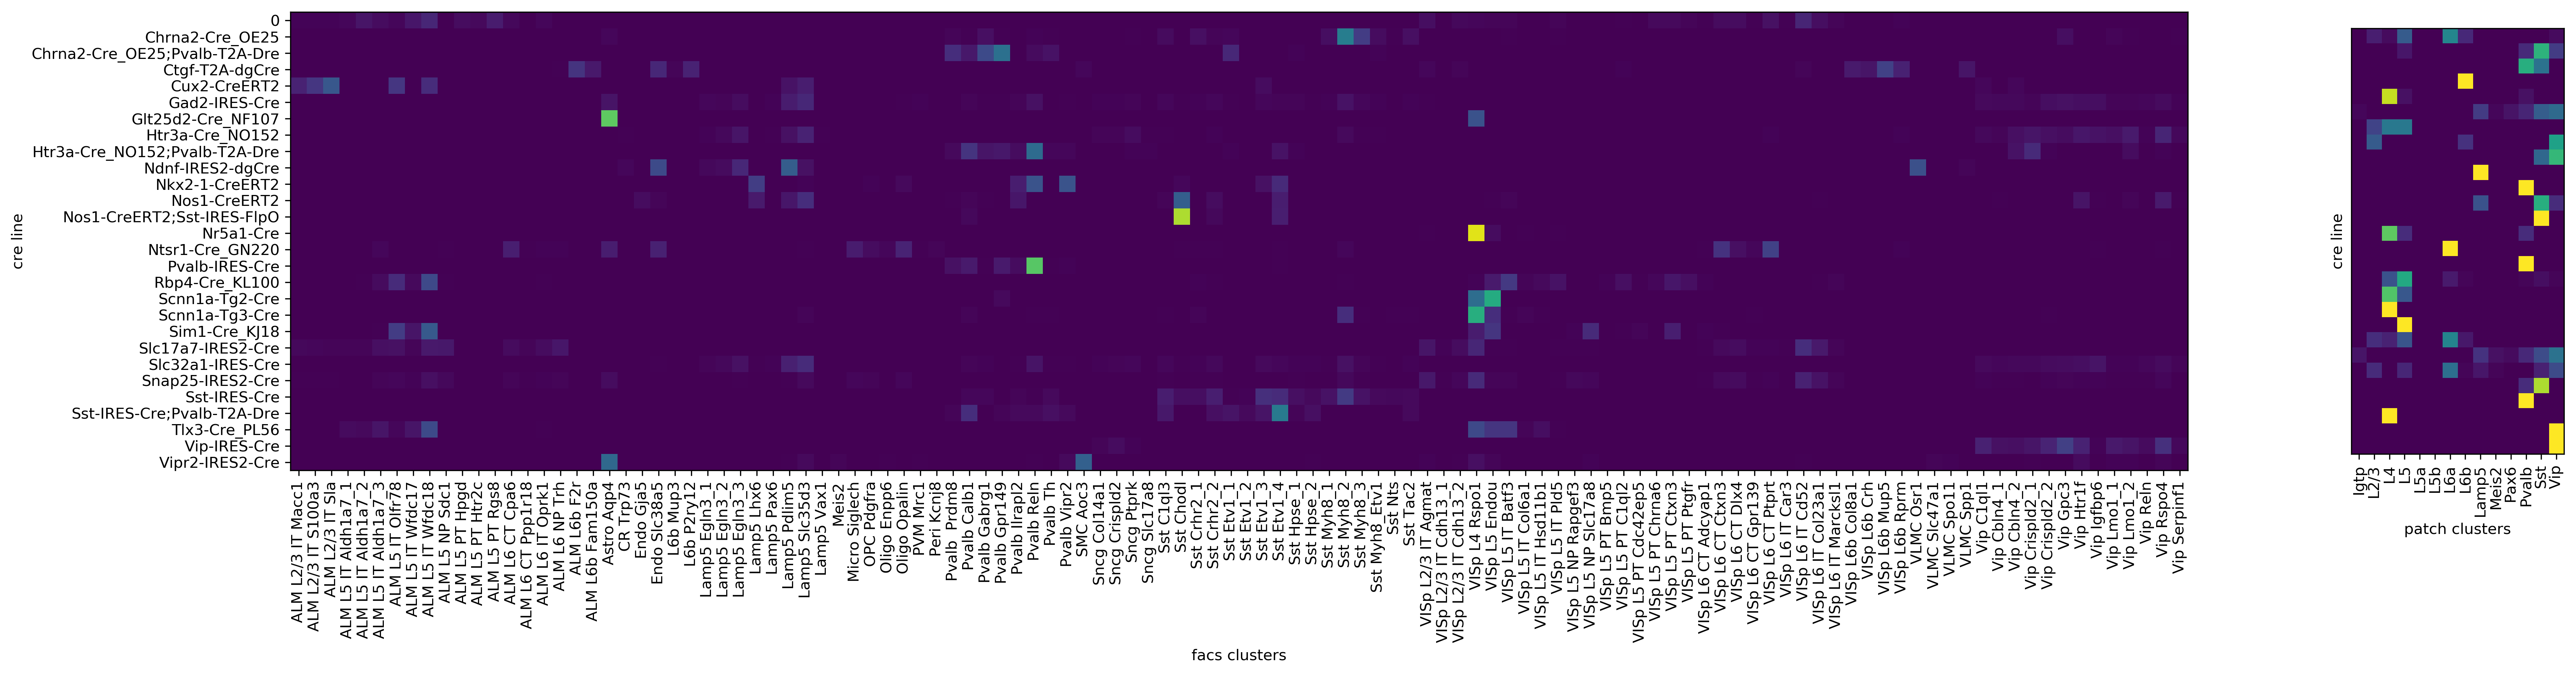
\includegraphics[width=.9\textheight,angle=270]{pics/alleninput}
\caption{Allen institute data: Our input \label{fig:alleninput}}
\end{figure}


\begin{figure}
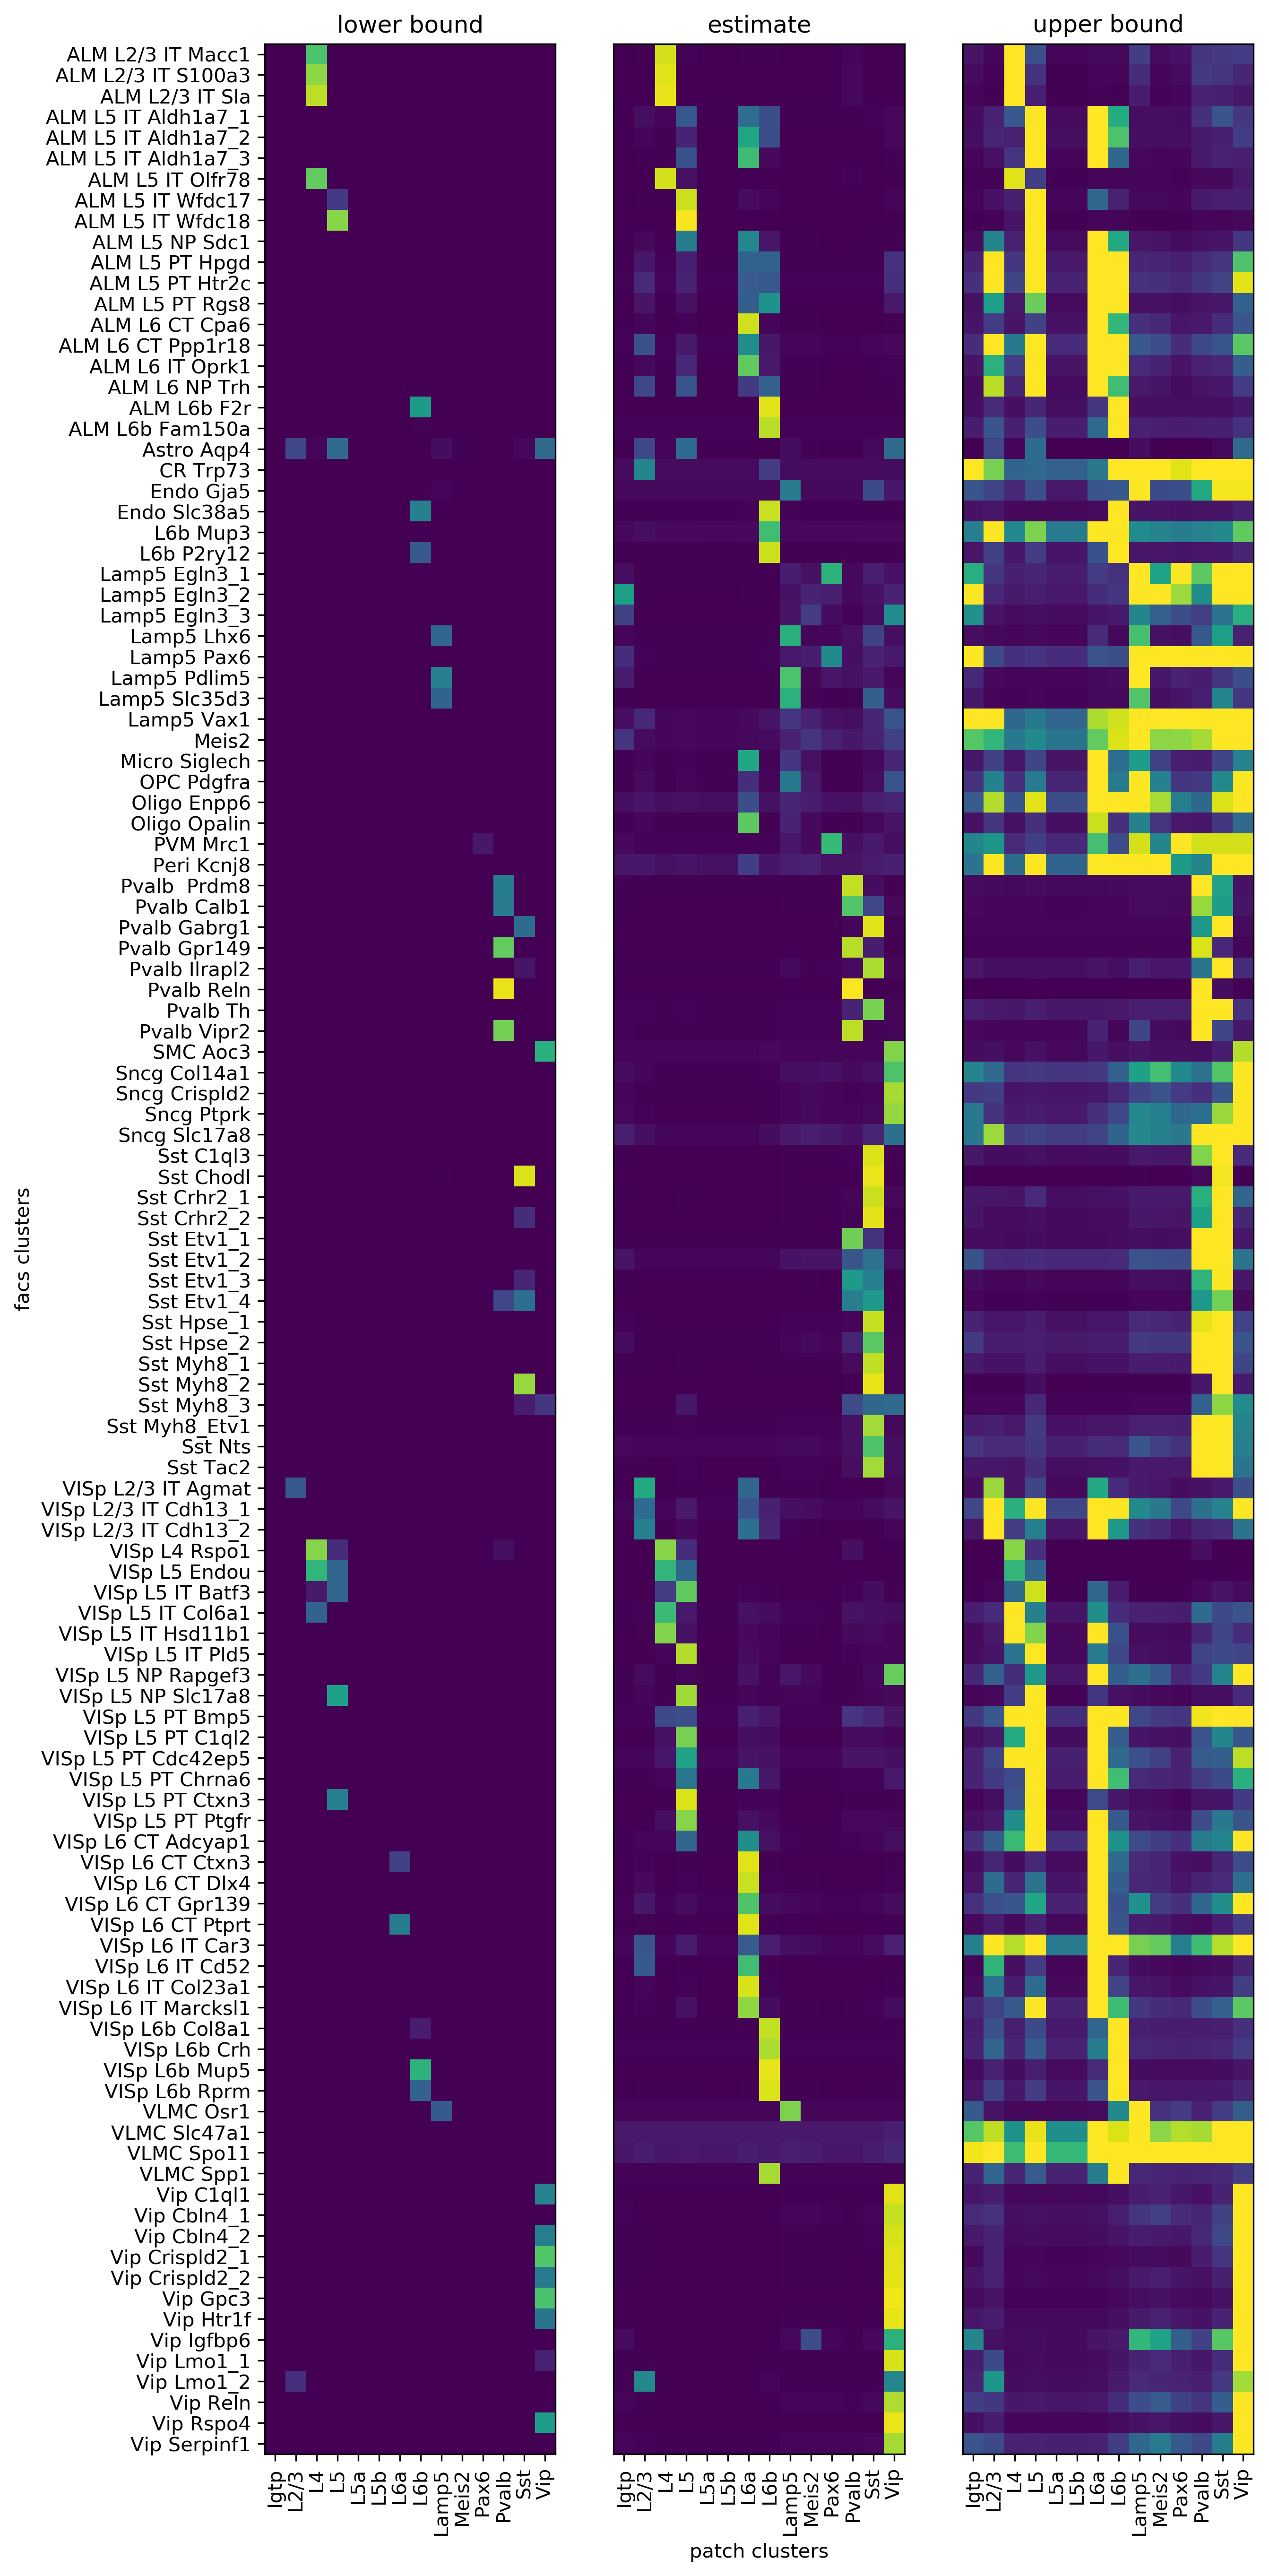
\includegraphics[width=0.8\textwidth]{pics/allen}
\caption{Allen institute data: Our output \label{fig:allenoutput}}
\end{figure}

These looked reasonable to the scientists, and also pointed out some possible issues.  In particular, some cell types tend to die more often in one experimental modality than another, which would violate our assumptions.  However, this doesn't bother them, because they see this technique as a way to \emph{validate} their assignments of clusters.  As such, if the result of our algorithm doesn't make sense, that's great because it may help them to figure out \emph{which cell types are dying more} and then they can upweight certain groups correspondingly.  Or it may help them figure out that their cluster assignment was all wrong.  This is how they see my method fitting into their pipelines: as a way of sanity checking their cluster assignments.  Which seems cool.

There is one possibly confusing aspect of our output that we would like to to address.  The upper and lower bounds (as we have visualized them) are each actually impossible as values for $q$.  For example, the rows of the upper bounds generally sum to more than 1.  This is because we have taken \emph{elementwise bounds} on each entry.  An alternative is to  sample uniformly from the set of possible values of $q$ which are consistent with our observations.  We hope this may give the user another way to understand what possible values $q$ might take on.  

To this end, we use a Dikin ellipsoid sampler to approximate uniform samples from the set of valid $q$s which are consistent with what we've observed.  These are shown in Figure \ref{fig:allenavg}.  Whether the MCMC method is mixing or not is of course up for debate.  See Appendix \ref{sec:dikin} for some details.

\begin{figure}
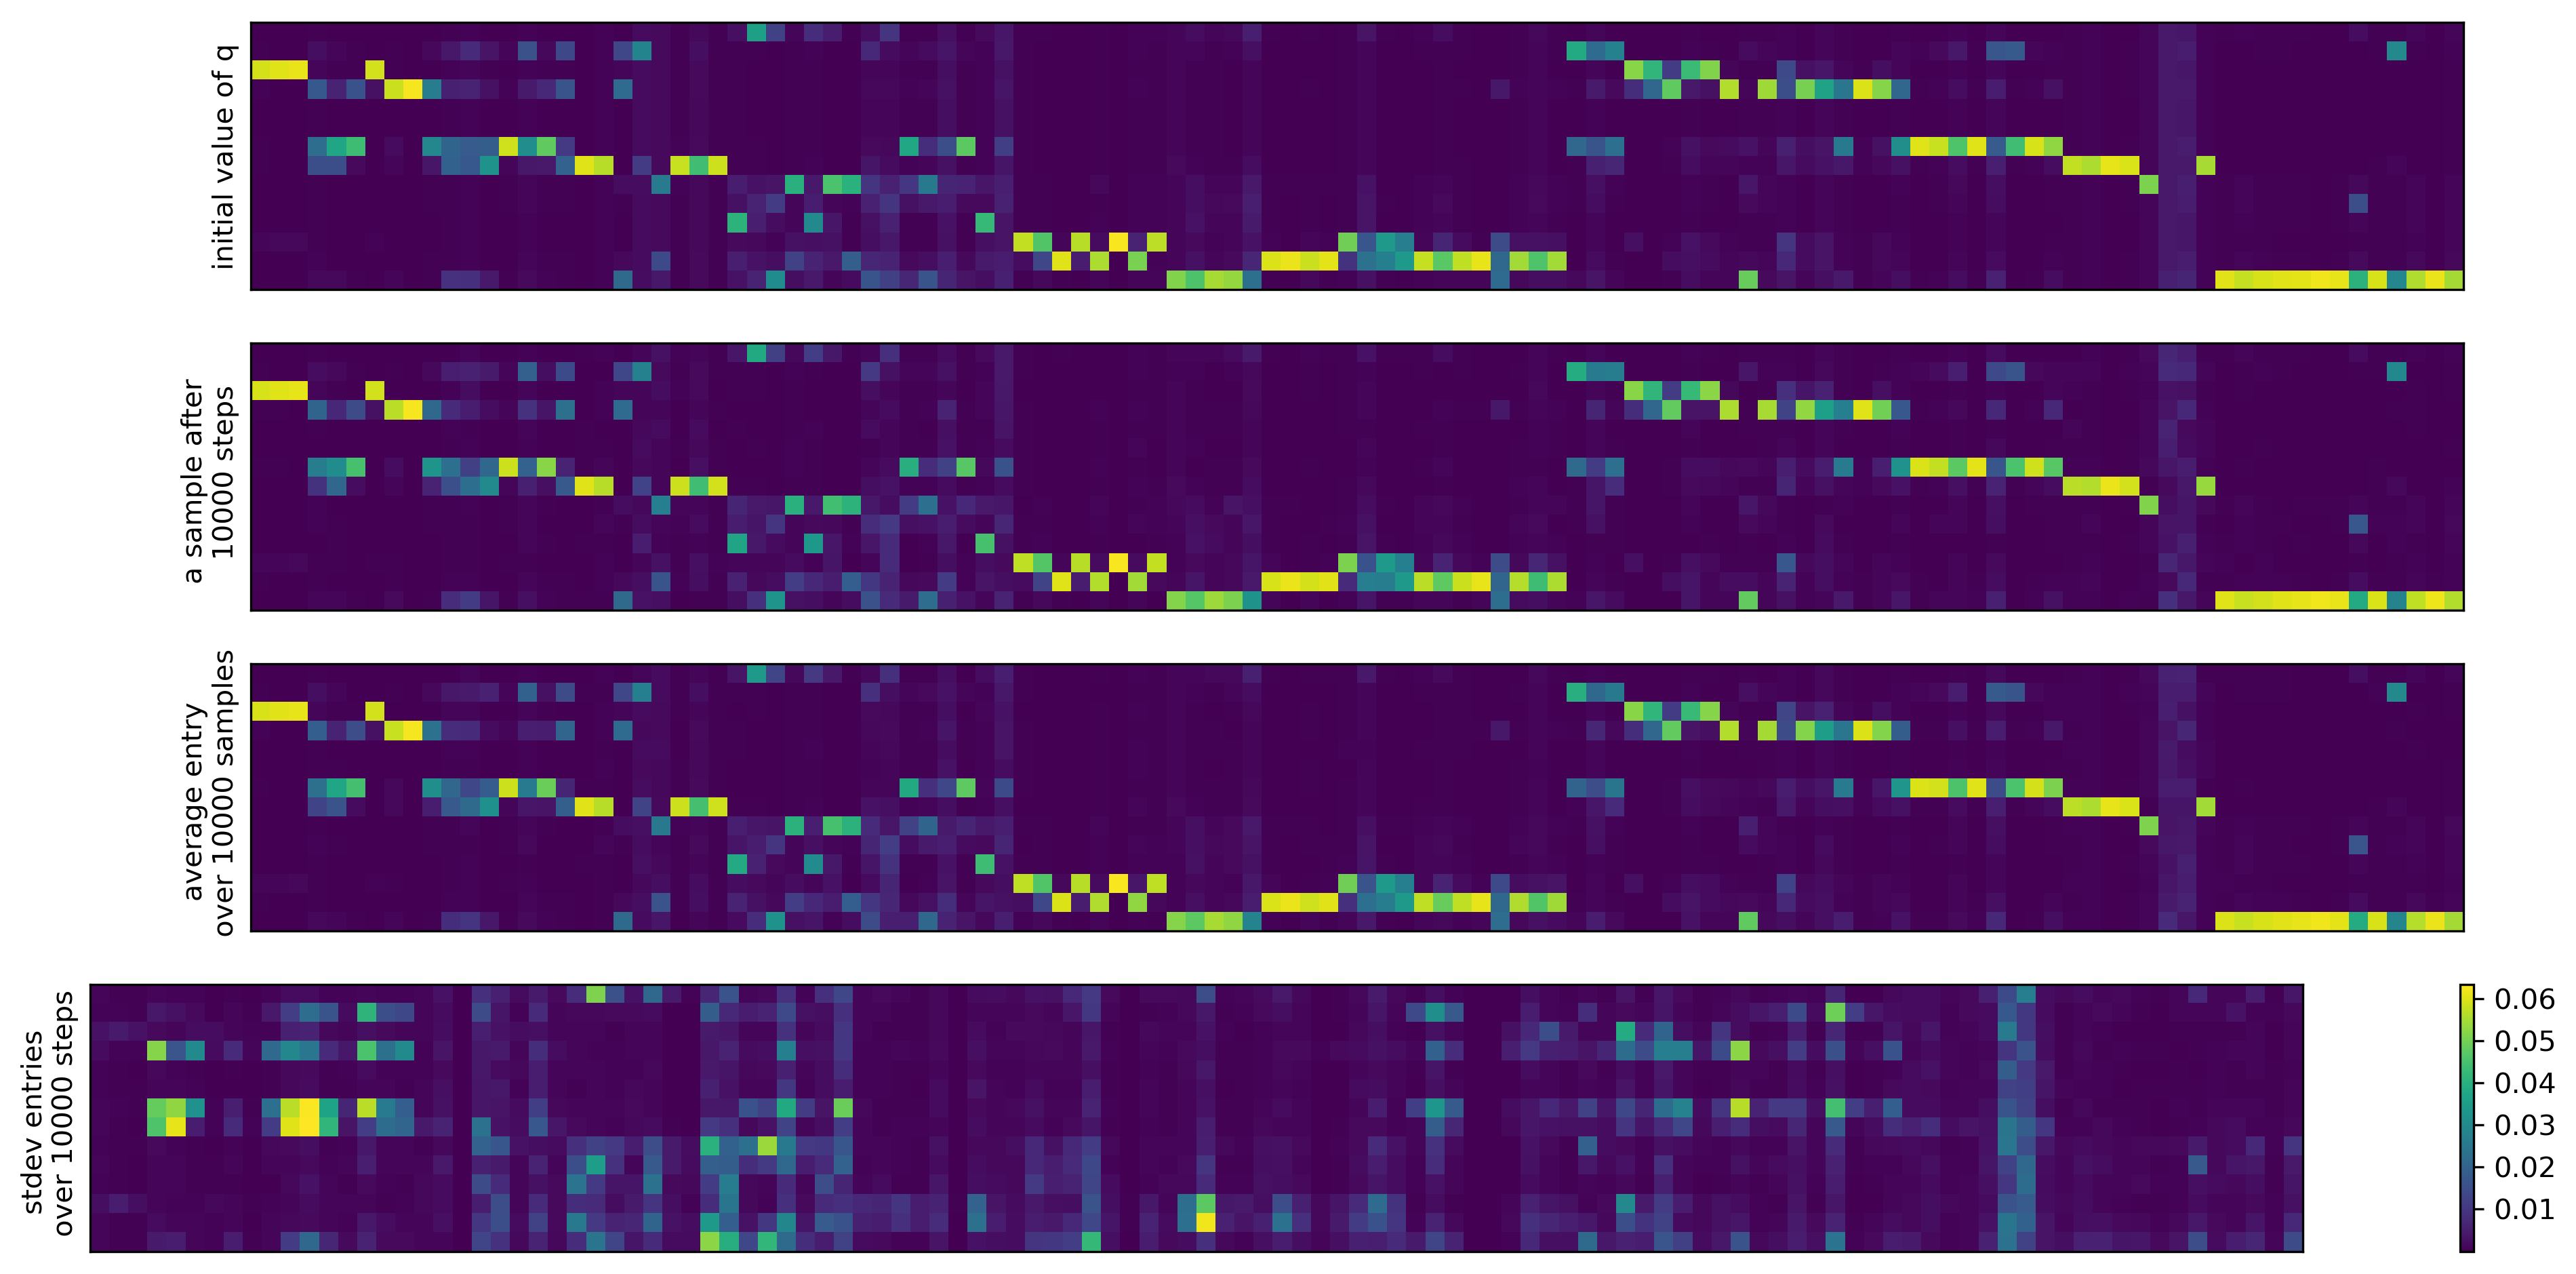
\includegraphics[width=0.8\textwidth]{pics/allenavg}
\caption{Allen institute data: sampling information.  The first plot is the estimated $q(y|x)$, as we have already seen in other figures.  The second plot is a single sample of $q(y|x)$,  The third plot is an average value of each entry of $q$ over many samples.  The final plot indicates the standard deviation of each entry over the samples. \label{fig:allenavg}}
\end{figure}

\section{The conjecture}

Here we give an outline for how the conjecture might be proved.

For any transition matrices $p,h$,\footnote{Here by transition matrix we just mean that the rows sum to 1 and the entries are nonnegative.} let $\Theta(p,h)$ denote the subset of transition matrices satisfying

\[
\Theta(p,h) \triangleq \{q:\ pq=h\}
\]

Now let us say we have some $p^*,h^*$, and some estimators $\hat p,\hat h$.  If the estimators were consistent, we might hope that $\Theta(\hat p,\hat h)$ would yield a consistent estimator for $\Theta(p^*,h^*)$.  In particular, we would ask that the Hausdorff distance would converge to zero in probability, $d_H(\Theta(\hat p,\hat h),\Theta(p^*,h^*))\rightarrow 0$.  Unfortunately, this is simply not the case.  Here's an example:

\begin{align*}
p^* &= (1, 0)\\
h^* &= (1, 0)\\
\Theta(p^*,h^*) &= 
  \left\{q:\ q=\left(\begin{array}{cc}
  1 & 0 \\
  \alpha & 1-\alpha \\
  \end{array}\right)\right\}
\end{align*}

Notice that the second row of $q$ is left \emph{totally} unspecified.  This is because the equation $p^*q=h^*$ simply places no constraints on the second row of $q$.  Now let us say we use our consistent estimator, and get something \emph{very} close to the truth.  We might get a dreadfully wrong impression of $q$:

\begin{align*}
\hat p &= \left(\frac{99}{100}, \frac{1}{100}\right)\\
\hat h &= (1, 0)\\
\Theta(\hat p,\hat h) &= 
  \left\{q:\ q=\left(\begin{array}{cc}
  1 & 0 \\
  1 & 0 \\
  \end{array}\right)\right\}
\end{align*}

Suddenly $q$ is \emph{entirely constrained} by the equation $pq=h$.  This dramatic change is possible because $q$ is constrained not only by the equation $pq=h$ but also by the fact that $q$ must be a transition matrix.  This allows for the possibility that although $p^*\approx \hat p$ and $h^*=\hat h$, we have that $d_H(\Theta(\hat p,\hat h),\Theta(p^*,h^*))=1$.  Not good.

However, this troubling example relied crucially on the fact that a given entry of $p$ went from zero to nonzero.  Let us therefore ask that the estimator $\hat p$ was consistent both in the usual Euclidean $\mathscr L^2$ sense, as well as in the sense that it eventually got the zeros right.  That is, $\mathbb P(\hat p(x|\ell)=0\Leftrightarrow p^*(x|\ell)=0) \rightarrow 1$.  Such an estimator is certainly easy to come by (the empirical distribution will do).  To prove consistency, it would then be sufficient to show that

\vspace{.1in}
\begin{conj}
For every $\epsilon>0$, we can find a $\delta>0$ so that if $|h_1 -h_2|^2<\delta$, $|p_1 -p_2|^2<\delta$, and $p_1(x|\ell)=0\Leftrightarrow p_2(x|\ell)=0$, then $d_H(\Theta(p_1,h_1),\Theta(p_1,h_1))<\epsilon$.
\end{conj}

To prove this conjecture, the essential point is to understand how the constraint $pq=h$ related to the $k$-faces (vertices, facets, etc) of the polytope of transition matrices.  If that constraint is somehow \emph{degenerate} with respect to one of the faces, then we get in trouble because a slight perturbation can change the degeneracy and thus create weird effects.  However, as long as the nature of the degeneracy is the same for both $p_1,p_2$, I believe there is no problem.  So to prove this conjecture, it remains to do three essential things

\begin{itemize}
    \item mathematically characterize the ``degeneracy'' of the constraint $pq=h$ with respect to faces of the transition matrix polytope
    \item show that if $p_1,p_2$ share the same qualitative nature of degeneracy and $p_1\approx p_2$, then $\Theta(p_1,h_1)\approx\Theta(p_2,h_2)$.
    \item show that the qualitative nature of this degeneracy is only changed when an entry of $p$ switches between zero and nonzero
\end{itemize}

\bibliographystyle{unsrt}
\bibliography{refs}

\appendix

\section{Dikin sampler}

\label{sec:dikin}

Consider a convex polytope $T=\{x:\ Ax\leq b\}$.  We have implemented a method for sampling from this polytope, based on the paper \citep{kannan2012random}.  This method makes use of the Dikin ellipsoids, $E(x)$.  For any $x$, these are defined by 

\begin{itemize}
    \item Computing the distance from $x$ to each facet of the polytope, i.e. $d_i = b_i - \sum_j A_{ij} X_j$.
    \item Constructing $\tilde A$ as $\tilde A_{ij} = A_{ij} / d_i$.
    \item Define $E(x) = \{y:\ |\tilde A (X-y)|\leq 1\}$.  
\end{itemize}

We can use these ellpsoids to efficiently sample the polytope $T$.    At each step, we have some point $X\in T$, and we would to use this point to obtain a new sample $Y$, such that by iterating this process we asymptotically obtain samples which are uniform in $T$.  Here is how we use $X$ to get $Y$:

\begin{algorithm}[H]
 \KwData{A point $X\in T$}
 \KwResult{A point $Y\in T$}
 \vspace{.1in}
  Sample a proposal $\tilde Y$, uniformly from $E(X)$\;
    \eIf{$X \in E(\tilde Y)$}{
        Sample $U \sim \mathrm{Uniform}[0,1]$\;
        \eIf{$U \leq \mathrm{Vol}(E(X))/\mathrm{Vol}(E(\tilde Y)) \leq 1$}{
            Let $Y \gets \tilde Y$\;
        }{
            Let $Y \gets X$\;
        }
    }{
        Let $Y\gets X$\;
    }
 \caption{Dikin sampler step}
\end{algorithm}

It is easy to show that the stationary distribution of the Markov chain found by iterating these Dikin sampler steps is indeed uniform on $T$.  To ensure an numerically robust method in the face of high-dimensional and nearly degenerate matrices, we take the following approach to robustly sampling from the ellipsoid:

\begin{algorithm}[H]
 \KwData{An $n\times m$ matrix $\tilde A$}
 \KwResult{A point $X$ sampled uniformly from $\{x:\ |Ax|\leq 1\}$}
 \vspace{.1in}
  Sample $Z$ as an $n$-dimensional normal variables vector\;
  Let $X$ denote the solution to the least squares problem $\min_x|\tilde Ax - Z|$\;
  Normalize $X$ by $X \gets X/|\tilde AX|$\;
  Sample $U \sim \mathrm{Uniform}[0,1]$\;
  Scale $X$ by $X \gets X \times U^{1/m}$\;
 \caption{Ellipsoid sampler}
\end{algorithm}


\end{document}






































